% Options for packages loaded elsewhere
\PassOptionsToPackage{unicode}{hyperref}
\PassOptionsToPackage{hyphens}{url}
%
\documentclass[
]{article}
\usepackage{amsmath,amssymb}
\usepackage{iftex}
\ifPDFTeX
  \usepackage[T1]{fontenc}
  \usepackage[utf8]{inputenc}
  \usepackage{textcomp} % provide euro and other symbols
\else % if luatex or xetex
  \usepackage{unicode-math} % this also loads fontspec
  \defaultfontfeatures{Scale=MatchLowercase}
  \defaultfontfeatures[\rmfamily]{Ligatures=TeX,Scale=1}
\fi
\usepackage{lmodern}
\ifPDFTeX\else
  % xetex/luatex font selection
\fi
% Use upquote if available, for straight quotes in verbatim environments
\IfFileExists{upquote.sty}{\usepackage{upquote}}{}
\IfFileExists{microtype.sty}{% use microtype if available
  \usepackage[]{microtype}
  \UseMicrotypeSet[protrusion]{basicmath} % disable protrusion for tt fonts
}{}
\makeatletter
\@ifundefined{KOMAClassName}{% if non-KOMA class
  \IfFileExists{parskip.sty}{%
    \usepackage{parskip}
  }{% else
    \setlength{\parindent}{0pt}
    \setlength{\parskip}{6pt plus 2pt minus 1pt}}
}{% if KOMA class
  \KOMAoptions{parskip=half}}
\makeatother
\usepackage{xcolor}
\usepackage[margin=1in]{geometry}
\usepackage{color}
\usepackage{fancyvrb}
\newcommand{\VerbBar}{|}
\newcommand{\VERB}{\Verb[commandchars=\\\{\}]}
\DefineVerbatimEnvironment{Highlighting}{Verbatim}{commandchars=\\\{\}}
% Add ',fontsize=\small' for more characters per line
\usepackage{framed}
\definecolor{shadecolor}{RGB}{248,248,248}
\newenvironment{Shaded}{\begin{snugshade}}{\end{snugshade}}
\newcommand{\AlertTok}[1]{\textcolor[rgb]{0.94,0.16,0.16}{#1}}
\newcommand{\AnnotationTok}[1]{\textcolor[rgb]{0.56,0.35,0.01}{\textbf{\textit{#1}}}}
\newcommand{\AttributeTok}[1]{\textcolor[rgb]{0.13,0.29,0.53}{#1}}
\newcommand{\BaseNTok}[1]{\textcolor[rgb]{0.00,0.00,0.81}{#1}}
\newcommand{\BuiltInTok}[1]{#1}
\newcommand{\CharTok}[1]{\textcolor[rgb]{0.31,0.60,0.02}{#1}}
\newcommand{\CommentTok}[1]{\textcolor[rgb]{0.56,0.35,0.01}{\textit{#1}}}
\newcommand{\CommentVarTok}[1]{\textcolor[rgb]{0.56,0.35,0.01}{\textbf{\textit{#1}}}}
\newcommand{\ConstantTok}[1]{\textcolor[rgb]{0.56,0.35,0.01}{#1}}
\newcommand{\ControlFlowTok}[1]{\textcolor[rgb]{0.13,0.29,0.53}{\textbf{#1}}}
\newcommand{\DataTypeTok}[1]{\textcolor[rgb]{0.13,0.29,0.53}{#1}}
\newcommand{\DecValTok}[1]{\textcolor[rgb]{0.00,0.00,0.81}{#1}}
\newcommand{\DocumentationTok}[1]{\textcolor[rgb]{0.56,0.35,0.01}{\textbf{\textit{#1}}}}
\newcommand{\ErrorTok}[1]{\textcolor[rgb]{0.64,0.00,0.00}{\textbf{#1}}}
\newcommand{\ExtensionTok}[1]{#1}
\newcommand{\FloatTok}[1]{\textcolor[rgb]{0.00,0.00,0.81}{#1}}
\newcommand{\FunctionTok}[1]{\textcolor[rgb]{0.13,0.29,0.53}{\textbf{#1}}}
\newcommand{\ImportTok}[1]{#1}
\newcommand{\InformationTok}[1]{\textcolor[rgb]{0.56,0.35,0.01}{\textbf{\textit{#1}}}}
\newcommand{\KeywordTok}[1]{\textcolor[rgb]{0.13,0.29,0.53}{\textbf{#1}}}
\newcommand{\NormalTok}[1]{#1}
\newcommand{\OperatorTok}[1]{\textcolor[rgb]{0.81,0.36,0.00}{\textbf{#1}}}
\newcommand{\OtherTok}[1]{\textcolor[rgb]{0.56,0.35,0.01}{#1}}
\newcommand{\PreprocessorTok}[1]{\textcolor[rgb]{0.56,0.35,0.01}{\textit{#1}}}
\newcommand{\RegionMarkerTok}[1]{#1}
\newcommand{\SpecialCharTok}[1]{\textcolor[rgb]{0.81,0.36,0.00}{\textbf{#1}}}
\newcommand{\SpecialStringTok}[1]{\textcolor[rgb]{0.31,0.60,0.02}{#1}}
\newcommand{\StringTok}[1]{\textcolor[rgb]{0.31,0.60,0.02}{#1}}
\newcommand{\VariableTok}[1]{\textcolor[rgb]{0.00,0.00,0.00}{#1}}
\newcommand{\VerbatimStringTok}[1]{\textcolor[rgb]{0.31,0.60,0.02}{#1}}
\newcommand{\WarningTok}[1]{\textcolor[rgb]{0.56,0.35,0.01}{\textbf{\textit{#1}}}}
\usepackage{graphicx}
\makeatletter
\def\maxwidth{\ifdim\Gin@nat@width>\linewidth\linewidth\else\Gin@nat@width\fi}
\def\maxheight{\ifdim\Gin@nat@height>\textheight\textheight\else\Gin@nat@height\fi}
\makeatother
% Scale images if necessary, so that they will not overflow the page
% margins by default, and it is still possible to overwrite the defaults
% using explicit options in \includegraphics[width, height, ...]{}
\setkeys{Gin}{width=\maxwidth,height=\maxheight,keepaspectratio}
% Set default figure placement to htbp
\makeatletter
\def\fps@figure{htbp}
\makeatother
\setlength{\emergencystretch}{3em} % prevent overfull lines
\providecommand{\tightlist}{%
  \setlength{\itemsep}{0pt}\setlength{\parskip}{0pt}}
\setcounter{secnumdepth}{5}
\usepackage{booktabs}
\usepackage{longtable}
\usepackage{array}
\usepackage{multirow}
\usepackage{wrapfig}
\usepackage{float}
\usepackage{colortbl}
\usepackage{pdflscape}
\usepackage{tabu}
\usepackage{threeparttable}
\usepackage{threeparttablex}
\usepackage[normalem]{ulem}
\usepackage{makecell}
\usepackage{xcolor}
\ifLuaTeX
  \usepackage{selnolig}  % disable illegal ligatures
\fi
\usepackage[]{natbib}
\bibliographystyle{plainnat}
\usepackage{bookmark}
\IfFileExists{xurl.sty}{\usepackage{xurl}}{} % add URL line breaks if available
\urlstyle{same}
\hypersetup{
  pdftitle={Causal Inference with Continuous Exposures: A Tutorial with Application to ICU Data: Real Data Analysis},
  pdfauthor={M Ehsan Karim},
  hidelinks,
  pdfcreator={LaTeX via pandoc}}

\title{Causal Inference with Continuous Exposures: A Tutorial with
Application to ICU Data: Real Data Analysis}
\author{M Ehsan Karim}
\date{}

\begin{document}
\maketitle

\subsection{Download and Prepare RHC
Data}\label{download-and-prepare-rhc-data}

\begin{Shaded}
\begin{Highlighting}[]
\CommentTok{\# Download data}
\NormalTok{ObsData }\OtherTok{\textless{}{-}} \FunctionTok{read.csv}\NormalTok{(}\StringTok{"https://hbiostat.org/data/repo/rhc.csv"}\NormalTok{, }\AttributeTok{header =} \ConstantTok{TRUE}\NormalTok{)}

\CommentTok{\# Calculate Length of Stay}
\NormalTok{ObsData}\SpecialCharTok{$}\NormalTok{Length.of.Stay }\OtherTok{\textless{}{-}}\NormalTok{ ObsData}\SpecialCharTok{$}\NormalTok{dschdte }\SpecialCharTok{{-}}\NormalTok{ ObsData}\SpecialCharTok{$}\NormalTok{sadmdte}
\NormalTok{ObsData}\SpecialCharTok{$}\NormalTok{Length.of.Stay[}\FunctionTok{is.na}\NormalTok{(ObsData}\SpecialCharTok{$}\NormalTok{Length.of.Stay)] }\OtherTok{\textless{}{-}} 
\NormalTok{  ObsData}\SpecialCharTok{$}\NormalTok{dthdte[}\FunctionTok{is.na}\NormalTok{(ObsData}\SpecialCharTok{$}\NormalTok{Length.of.Stay)] }\SpecialCharTok{{-}} 
\NormalTok{  ObsData}\SpecialCharTok{$}\NormalTok{sadmdte[}\FunctionTok{is.na}\NormalTok{(ObsData}\SpecialCharTok{$}\NormalTok{Length.of.Stay)]}

\CommentTok{\# Binary outcome}
\NormalTok{ObsData}\SpecialCharTok{$}\NormalTok{death }\OtherTok{\textless{}{-}} \FunctionTok{ifelse}\NormalTok{(ObsData}\SpecialCharTok{$}\NormalTok{death }\SpecialCharTok{==} \StringTok{"Yes"}\NormalTok{, }\DecValTok{1}\NormalTok{, }\DecValTok{0}\NormalTok{)}

\CommentTok{\# Remove unwanted outcome variables}
\NormalTok{ObsData }\OtherTok{\textless{}{-}}\NormalTok{ dplyr}\SpecialCharTok{::}\FunctionTok{select}\NormalTok{(ObsData, }\SpecialCharTok{!}\FunctionTok{c}\NormalTok{(dthdte, }
\NormalTok{                                     lstctdte, }
\NormalTok{                                     dschdte, }
\NormalTok{                                     t3d30, }
\NormalTok{                                     dth30, }
\NormalTok{                                     surv2md1))}

\CommentTok{\# Remove problematic variables}
\NormalTok{ObsData }\OtherTok{\textless{}{-}}\NormalTok{ dplyr}\SpecialCharTok{::}\FunctionTok{select}\NormalTok{(ObsData, }\SpecialCharTok{!}\FunctionTok{c}\NormalTok{(sadmdte, }
\NormalTok{                                     ptid, }
\NormalTok{                                     X, }
\NormalTok{                                     adld3p, }
\NormalTok{                                     urin1, }
\NormalTok{                                     cat2))}

\CommentTok{\# Convert categorical variables}
\NormalTok{factors }\OtherTok{\textless{}{-}} \FunctionTok{c}\NormalTok{(}\StringTok{"cat1"}\NormalTok{, }\StringTok{"ca"}\NormalTok{, }\StringTok{"death"}\NormalTok{, }\StringTok{"cardiohx"}\NormalTok{, }\StringTok{"chfhx"}\NormalTok{, }\StringTok{"dementhx"}\NormalTok{, }\StringTok{"psychhx"}\NormalTok{, }
             \StringTok{"chrpulhx"}\NormalTok{, }\StringTok{"renalhx"}\NormalTok{, }\StringTok{"liverhx"}\NormalTok{, }\StringTok{"gibledhx"}\NormalTok{, }\StringTok{"malighx"}\NormalTok{, }\StringTok{"immunhx"}\NormalTok{, }
             \StringTok{"transhx"}\NormalTok{, }\StringTok{"amihx"}\NormalTok{, }\StringTok{"sex"}\NormalTok{, }\StringTok{"dnr1"}\NormalTok{, }\StringTok{"ninsclas"}\NormalTok{, }\StringTok{"resp"}\NormalTok{, }\StringTok{"card"}\NormalTok{, }\StringTok{"neuro"}\NormalTok{, }
             \StringTok{"gastr"}\NormalTok{, }\StringTok{"renal"}\NormalTok{, }\StringTok{"meta"}\NormalTok{, }\StringTok{"hema"}\NormalTok{, }\StringTok{"seps"}\NormalTok{, }\StringTok{"trauma"}\NormalTok{, }\StringTok{"ortho"}\NormalTok{, }\StringTok{"race"}\NormalTok{, }
             \StringTok{"income"}\NormalTok{)}
\NormalTok{ObsData[factors] }\OtherTok{\textless{}{-}} \FunctionTok{lapply}\NormalTok{(ObsData[factors], as.factor)}

\CommentTok{\# Recode RHC use}
\NormalTok{ObsData}\SpecialCharTok{$}\NormalTok{RHC.use }\OtherTok{\textless{}{-}} \FunctionTok{ifelse}\NormalTok{(ObsData}\SpecialCharTok{$}\NormalTok{swang1 }\SpecialCharTok{==} \StringTok{"RHC"}\NormalTok{, }\DecValTok{1}\NormalTok{, }\DecValTok{0}\NormalTok{)}
\NormalTok{ObsData }\OtherTok{\textless{}{-}}\NormalTok{ dplyr}\SpecialCharTok{::}\FunctionTok{select}\NormalTok{(ObsData, }\SpecialCharTok{{-}}\NormalTok{swang1)}

\CommentTok{\# Recode and factor levels}
\NormalTok{ObsData}\SpecialCharTok{$}\NormalTok{age }\OtherTok{\textless{}{-}} \FunctionTok{cut}\NormalTok{(ObsData}\SpecialCharTok{$}\NormalTok{age, }\AttributeTok{breaks=}\FunctionTok{c}\NormalTok{(}\SpecialCharTok{{-}}\ConstantTok{Inf}\NormalTok{, }\DecValTok{50}\NormalTok{, }\DecValTok{60}\NormalTok{, }\DecValTok{70}\NormalTok{, }\DecValTok{80}\NormalTok{, }\ConstantTok{Inf}\NormalTok{), }\AttributeTok{right=}\ConstantTok{FALSE}\NormalTok{)}
\NormalTok{ObsData}\SpecialCharTok{$}\NormalTok{race }\OtherTok{\textless{}{-}} \FunctionTok{factor}\NormalTok{(ObsData}\SpecialCharTok{$}\NormalTok{race, }\AttributeTok{levels=}\FunctionTok{c}\NormalTok{(}\StringTok{"white"}\NormalTok{, }\StringTok{"black"}\NormalTok{, }\StringTok{"other"}\NormalTok{))}
\NormalTok{ObsData}\SpecialCharTok{$}\NormalTok{sex }\OtherTok{\textless{}{-}} \FunctionTok{relevel}\NormalTok{(}\FunctionTok{as.factor}\NormalTok{(ObsData}\SpecialCharTok{$}\NormalTok{sex), }\AttributeTok{ref =} \StringTok{"Male"}\NormalTok{)}
\NormalTok{ObsData}\SpecialCharTok{$}\NormalTok{cat1 }\OtherTok{\textless{}{-}} \FunctionTok{factor}\NormalTok{(ObsData}\SpecialCharTok{$}\NormalTok{cat1, }\AttributeTok{levels =} \FunctionTok{unique}\NormalTok{(ObsData}\SpecialCharTok{$}\NormalTok{cat1))}
\FunctionTok{levels}\NormalTok{(ObsData}\SpecialCharTok{$}\NormalTok{cat1) }\OtherTok{\textless{}{-}} \FunctionTok{c}\NormalTok{(}\StringTok{"ARF"}\NormalTok{, }\StringTok{"CHF"}\NormalTok{, }\StringTok{"Other"}\NormalTok{, }\StringTok{"Other"}\NormalTok{, }\StringTok{"Other"}\NormalTok{, }\StringTok{"Other"}\NormalTok{, }\StringTok{"Other"}\NormalTok{, }\StringTok{"MOSF"}\NormalTok{, }\StringTok{"MOSF"}\NormalTok{)}
\NormalTok{ObsData}\SpecialCharTok{$}\NormalTok{ca }\OtherTok{\textless{}{-}} \FunctionTok{factor}\NormalTok{(ObsData}\SpecialCharTok{$}\NormalTok{ca, }\AttributeTok{levels =} \FunctionTok{c}\NormalTok{(}\StringTok{"No"}\NormalTok{, }\StringTok{"Yes"}\NormalTok{), }\AttributeTok{labels =} \FunctionTok{c}\NormalTok{(}\StringTok{"None"}\NormalTok{, }\StringTok{"Metastatic"}\NormalTok{))}

\CommentTok{\# Rename variables}
\FunctionTok{names}\NormalTok{(ObsData) }\OtherTok{\textless{}{-}} \FunctionTok{c}\NormalTok{(}\StringTok{"Disease.category"}\NormalTok{, }\StringTok{"Cancer"}\NormalTok{, }\StringTok{"Death"}\NormalTok{, }\StringTok{"Cardiovascular"}\NormalTok{, }\StringTok{"Congestive.HF"}\NormalTok{, }
                    \StringTok{"Dementia"}\NormalTok{, }\StringTok{"Psychiatric"}\NormalTok{, }\StringTok{"Pulmonary"}\NormalTok{, }\StringTok{"Renal"}\NormalTok{, }\StringTok{"Hepatic"}\NormalTok{, }\StringTok{"GI.Bleed"}\NormalTok{, }
                    \StringTok{"Tumor"}\NormalTok{, }\StringTok{"Immunosupperssion"}\NormalTok{, }\StringTok{"Transfer.hx"}\NormalTok{, }\StringTok{"MI"}\NormalTok{, }\StringTok{"age"}\NormalTok{, }\StringTok{"sex"}\NormalTok{, }\StringTok{"edu"}\NormalTok{, }
                    \StringTok{"DASIndex"}\NormalTok{, }\StringTok{"APACHE.score"}\NormalTok{, }\StringTok{"Glasgow.Coma.Score"}\NormalTok{, }\StringTok{"blood.pressure"}\NormalTok{, }\StringTok{"WBC"}\NormalTok{, }
                    \StringTok{"Heart.rate"}\NormalTok{, }\StringTok{"Respiratory.rate"}\NormalTok{, }\StringTok{"Temperature"}\NormalTok{, }\StringTok{"PaO2vs.FIO2"}\NormalTok{, }\StringTok{"Albumin"}\NormalTok{, }
                    \StringTok{"Hematocrit"}\NormalTok{, }\StringTok{"Bilirubin"}\NormalTok{, }\StringTok{"Creatinine"}\NormalTok{, }\StringTok{"Sodium"}\NormalTok{, }\StringTok{"Potassium"}\NormalTok{, }\StringTok{"PaCo2"}\NormalTok{, }
                    \StringTok{"PH"}\NormalTok{, }\StringTok{"Weight"}\NormalTok{, }\StringTok{"DNR.status"}\NormalTok{, }\StringTok{"Medical.insurance"}\NormalTok{, }\StringTok{"Respiratory.Diag"}\NormalTok{, }
                    \StringTok{"Cardiovascular.Diag"}\NormalTok{, }\StringTok{"Neurological.Diag"}\NormalTok{, }\StringTok{"Gastrointestinal.Diag"}\NormalTok{, }
                    \StringTok{"Renal.Diag"}\NormalTok{, }\StringTok{"Metabolic.Diag"}\NormalTok{, }\StringTok{"Hematologic.Diag"}\NormalTok{, }\StringTok{"Sepsis.Diag"}\NormalTok{, }
                    \StringTok{"Trauma.Diag"}\NormalTok{, }\StringTok{"Orthopedic.Diag"}\NormalTok{, }\StringTok{"race"}\NormalTok{, }\StringTok{"income"}\NormalTok{, }\StringTok{"Length.of.Stay"}\NormalTok{, }
                    \StringTok{"RHC.use"}\NormalTok{)}

\FunctionTok{str}\NormalTok{(ObsData)}
\end{Highlighting}
\end{Shaded}

\begin{verbatim}
## 'data.frame':    5735 obs. of  52 variables:
##  $ Disease.category     : Factor w/ 4 levels "ARF","CHF","Other",..: 1 2 3 3 2 1 3 3 3 3 ...
##  $ Cancer               : Factor w/ 2 levels "None","Metastatic": 2 1 2 1 1 1 NA 1 2 2 ...
##  $ Death                : Factor w/ 2 levels "0","1": 1 2 1 2 2 1 1 2 1 1 ...
##  $ Cardiovascular       : Factor w/ 2 levels "0","1": 1 2 1 1 1 1 1 1 1 1 ...
##  $ Congestive.HF        : Factor w/ 2 levels "0","1": 1 2 1 1 1 2 1 1 1 1 ...
##  $ Dementia             : Factor w/ 2 levels "0","1": 1 1 1 1 1 1 1 1 1 1 ...
##  $ Psychiatric          : Factor w/ 2 levels "0","1": 1 1 1 1 1 1 1 1 1 1 ...
##  $ Pulmonary            : Factor w/ 2 levels "0","1": 2 1 1 1 1 2 1 1 1 1 ...
##  $ Renal                : Factor w/ 2 levels "0","1": 1 1 1 1 1 1 1 1 1 1 ...
##  $ Hepatic              : Factor w/ 2 levels "0","1": 1 1 1 1 1 1 1 1 1 1 ...
##  $ GI.Bleed             : Factor w/ 2 levels "0","1": 1 1 1 1 1 1 1 1 1 1 ...
##  $ Tumor                : Factor w/ 2 levels "0","1": 2 1 2 1 1 1 2 1 1 2 ...
##  $ Immunosupperssion    : Factor w/ 2 levels "0","1": 1 2 2 2 1 1 1 1 1 1 ...
##  $ Transfer.hx          : Factor w/ 2 levels "0","1": 1 2 1 1 1 1 1 2 1 1 ...
##  $ MI                   : Factor w/ 2 levels "0","1": 1 1 1 1 1 1 1 1 1 1 ...
##  $ age                  : Factor w/ 5 levels "[-Inf,50)","[50,60)",..: 4 4 1 4 3 5 2 1 1 1 ...
##  $ sex                  : Factor w/ 2 levels "Male","Female": 1 2 2 2 1 2 1 1 2 2 ...
##  $ edu                  : num  12 12 14.07 9 9.95 ...
##  $ DASIndex             : num  23.5 14.8 18.1 22.9 21.1 ...
##  $ APACHE.score         : int  46 50 82 48 72 38 29 25 47 48 ...
##  $ Glasgow.Coma.Score   : int  0 0 0 0 41 0 26 100 0 0 ...
##  $ blood.pressure       : num  41 63 57 55 65 115 67 128 53 73 ...
##  $ WBC                  : num  22.1 28.9 0.05 23.3 29.7 ...
##  $ Heart.rate           : int  124 137 130 58 125 134 135 102 118 141 ...
##  $ Respiratory.rate     : num  10 38 40 26 27 36 10 34 30 40 ...
##  $ Temperature          : num  38.7 38.9 36.4 35.8 34.8 ...
##  $ PaO2vs.FIO2          : num  68 218 276 157 478 ...
##  $ Albumin              : num  3.5 2.6 3.5 3.5 3.5 ...
##  $ Hematocrit           : num  58 32.5 21.1 26.3 24 ...
##  $ Bilirubin            : num  1.01 0.7 1.01 0.4 1.01 ...
##  $ Creatinine           : num  1.2 0.6 2.6 1.7 3.6 ...
##  $ Sodium               : int  145 137 146 117 126 138 136 136 136 146 ...
##  $ Potassium            : num  4 3.3 2.9 5.8 5.8 ...
##  $ PaCo2                : num  40 34 16 30 17 68 45 26 40 30 ...
##  $ PH                   : num  7.36 7.33 7.36 7.46 7.23 ...
##  $ Weight               : num  64.7 45.7 0 54.6 78.4 ...
##  $ DNR.status           : Factor w/ 2 levels "No","Yes": 1 1 1 1 2 1 1 1 1 1 ...
##  $ Medical.insurance    : Factor w/ 6 levels "Medicaid","Medicare",..: 2 6 5 6 2 2 5 5 5 1 ...
##  $ Respiratory.Diag     : Factor w/ 2 levels "No","Yes": 2 1 1 2 1 2 1 2 1 1 ...
##  $ Cardiovascular.Diag  : Factor w/ 2 levels "No","Yes": 2 1 2 1 2 1 1 1 1 1 ...
##  $ Neurological.Diag    : Factor w/ 2 levels "No","Yes": 1 1 1 1 1 1 1 2 1 2 ...
##  $ Gastrointestinal.Diag: Factor w/ 2 levels "No","Yes": 1 1 1 1 1 1 1 1 1 2 ...
##  $ Renal.Diag           : Factor w/ 2 levels "No","Yes": 1 1 1 1 1 1 2 1 1 1 ...
##  $ Metabolic.Diag       : Factor w/ 2 levels "No","Yes": 1 1 1 1 1 1 1 1 1 1 ...
##  $ Hematologic.Diag     : Factor w/ 2 levels "No","Yes": 1 1 1 1 1 1 1 1 2 1 ...
##  $ Sepsis.Diag          : Factor w/ 2 levels "No","Yes": 1 2 1 1 1 1 1 2 1 1 ...
##  $ Trauma.Diag          : Factor w/ 2 levels "No","Yes": 1 1 1 1 1 1 1 1 1 1 ...
##  $ Orthopedic.Diag      : Factor w/ 2 levels "No","Yes": 1 1 1 1 1 1 1 1 1 1 ...
##  $ race                 : Factor w/ 3 levels "white","black",..: 1 1 1 1 1 1 1 1 1 1 ...
##  $ income               : Factor w/ 4 levels "$11-$25k","$25-$50k",..: 4 4 2 1 4 4 2 2 4 4 ...
##  $ Length.of.Stay       : int  9 45 60 37 2 7 42 34 11 19 ...
##  $ RHC.use              : num  0 1 1 0 1 0 0 0 0 1 ...
\end{verbatim}

\begin{Shaded}
\begin{Highlighting}[]
\CommentTok{\# Save cleaned dataset}
\FunctionTok{saveRDS}\NormalTok{(ObsData, }\AttributeTok{file =} \StringTok{"rhcAnalytic.RDS"}\NormalTok{)}
\end{Highlighting}
\end{Shaded}

\subsection{Load RHC Data}\label{load-rhc-data}

\begin{Shaded}
\begin{Highlighting}[]
\NormalTok{rhc }\OtherTok{\textless{}{-}} \FunctionTok{readRDS}\NormalTok{(}\StringTok{"rhcAnalytic.RDS"}\NormalTok{)}

\CommentTok{\# Define comprehensive confounder set}
\NormalTok{covariates }\OtherTok{\textless{}{-}} \FunctionTok{c}\NormalTok{(}
  \StringTok{"age"}\NormalTok{, }\StringTok{"sex"}\NormalTok{, }\StringTok{"Cardiovascular"}\NormalTok{, }\StringTok{"Pulmonary"}\NormalTok{, }
  \StringTok{"Renal"}\NormalTok{, }\StringTok{"Congestive.HF"}\NormalTok{, }\StringTok{"Cancer"}\NormalTok{,}
  \StringTok{"APACHE.score"}\NormalTok{, }\StringTok{"DASIndex"}\NormalTok{, }\StringTok{"Albumin"}\NormalTok{, }
  \StringTok{"Creatinine"}\NormalTok{, }\StringTok{"Sodium"}\NormalTok{, }\StringTok{"Heart.rate"}\NormalTok{, }\StringTok{"WBC"}\NormalTok{,}
  \StringTok{"DNR.status"}\NormalTok{, }\StringTok{"Transfer.hx"}
\NormalTok{)}

\CommentTok{\# Prepare variables}
\NormalTok{rhc }\OtherTok{\textless{}{-}}\NormalTok{ rhc }\SpecialCharTok{\%\textgreater{}\%}
  \FunctionTok{mutate}\NormalTok{(}
    \AttributeTok{A =}\NormalTok{ blood.pressure,}
    \AttributeTok{Y =} \FunctionTok{as.numeric}\NormalTok{(}\FunctionTok{as.character}\NormalTok{(Death))}
\NormalTok{  ) }\SpecialCharTok{\%\textgreater{}\%}
  \FunctionTok{filter}\NormalTok{(}\SpecialCharTok{!}\FunctionTok{is.na}\NormalTok{(A), }\SpecialCharTok{!}\FunctionTok{is.na}\NormalTok{(Y)) }\SpecialCharTok{\%\textgreater{}\%}
  \FunctionTok{filter}\NormalTok{(}\FunctionTok{complete.cases}\NormalTok{(}\FunctionTok{select}\NormalTok{(., }\FunctionTok{all\_of}\NormalTok{(covariates))))}
\end{Highlighting}
\end{Shaded}

\subsection{Summarize the Exposure}\label{summarize-the-exposure}

\begin{Shaded}
\begin{Highlighting}[]
\FunctionTok{ggplot}\NormalTok{(rhc, }\FunctionTok{aes}\NormalTok{(}\AttributeTok{x =}\NormalTok{ A)) }\SpecialCharTok{+}
  \FunctionTok{geom\_histogram}\NormalTok{(}\FunctionTok{aes}\NormalTok{(}\AttributeTok{y =}\NormalTok{ ..density..), }\AttributeTok{bins =} \DecValTok{40}\NormalTok{, }\AttributeTok{fill =} \StringTok{"steelblue"}\NormalTok{, }\AttributeTok{alpha =} \FloatTok{0.6}\NormalTok{) }\SpecialCharTok{+}
  \FunctionTok{geom\_density}\NormalTok{(}\AttributeTok{color =} \StringTok{"black"}\NormalTok{, }\AttributeTok{linewidth =} \DecValTok{1}\NormalTok{) }\SpecialCharTok{+}
  \FunctionTok{labs}\NormalTok{(}
    \AttributeTok{title =} \StringTok{"Distribution of Blood Pressure (Exposure A)"}\NormalTok{,}
    \AttributeTok{x =} \StringTok{"Blood Pressure"}\NormalTok{,}
    \AttributeTok{y =} \StringTok{"Density"}
\NormalTok{  ) }\SpecialCharTok{+}
  \FunctionTok{theme\_minimal}\NormalTok{(}\AttributeTok{base\_size =} \DecValTok{13}\NormalTok{)}
\end{Highlighting}
\end{Shaded}

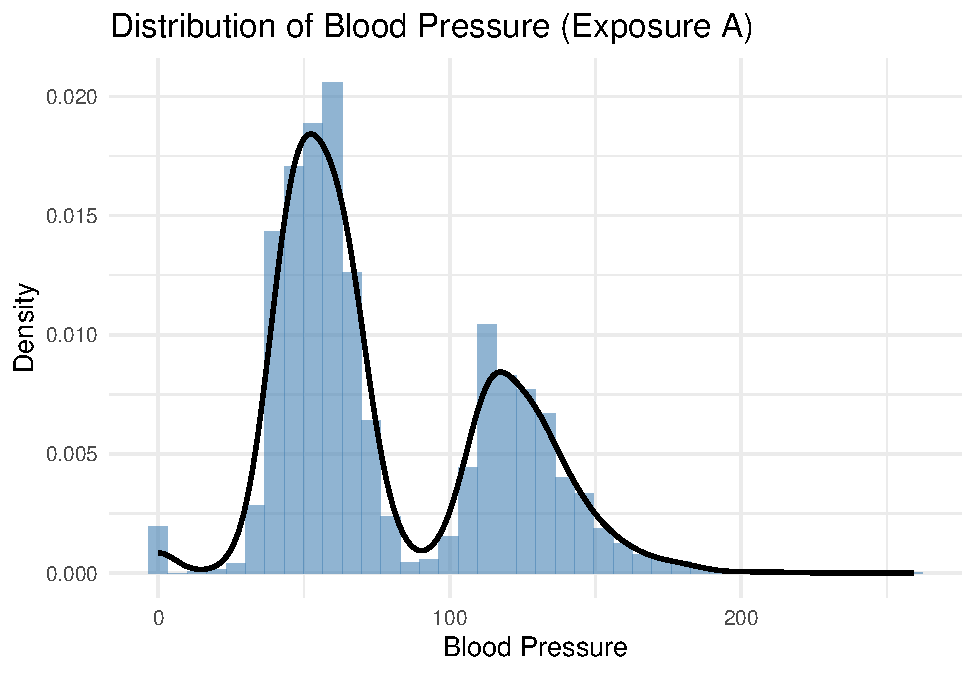
\includegraphics{rhc_analysis_files/figure-latex/plot-A-distribution-1.pdf}

\subsection{Method 1: IPW with Normal Exposure
Model}\label{method-1-ipw-with-normal-exposure-model}

\begin{Shaded}
\begin{Highlighting}[]
\CommentTok{\# Numerator: marginal exposure model}
\NormalTok{mod\_num }\OtherTok{\textless{}{-}} \FunctionTok{lm}\NormalTok{(A }\SpecialCharTok{\textasciitilde{}} \DecValTok{1}\NormalTok{, }\AttributeTok{data =}\NormalTok{ rhc)}
\NormalTok{mu\_num }\OtherTok{\textless{}{-}} \FunctionTok{predict}\NormalTok{(mod\_num)}
\NormalTok{sd\_num }\OtherTok{\textless{}{-}} \FunctionTok{sd}\NormalTok{(}\FunctionTok{residuals}\NormalTok{(mod\_num))}

\CommentTok{\# Denominator: exposure conditional on confounders}
\NormalTok{form\_denom }\OtherTok{\textless{}{-}} \FunctionTok{as.formula}\NormalTok{(}\FunctionTok{paste}\NormalTok{(}\StringTok{"A \textasciitilde{}"}\NormalTok{, }
                               \FunctionTok{paste}\NormalTok{(covariates, }\AttributeTok{collapse =} \StringTok{" + "}\NormalTok{)))}
\NormalTok{mod\_denom }\OtherTok{\textless{}{-}} \FunctionTok{lm}\NormalTok{(form\_denom, }\AttributeTok{data =}\NormalTok{ rhc)}
\NormalTok{mu\_denom }\OtherTok{\textless{}{-}} \FunctionTok{predict}\NormalTok{(mod\_denom)}
\NormalTok{sd\_denom }\OtherTok{\textless{}{-}} \FunctionTok{sd}\NormalTok{(}\FunctionTok{residuals}\NormalTok{(mod\_denom))}

\CommentTok{\# Densities and weights}
\NormalTok{f\_num }\OtherTok{\textless{}{-}} \FunctionTok{dnorm}\NormalTok{(rhc}\SpecialCharTok{$}\NormalTok{A, }\AttributeTok{mean =}\NormalTok{ mu\_num, }\AttributeTok{sd =}\NormalTok{ sd\_num)}
\NormalTok{f\_denom }\OtherTok{\textless{}{-}} \FunctionTok{dnorm}\NormalTok{(rhc}\SpecialCharTok{$}\NormalTok{A, }\AttributeTok{mean =}\NormalTok{ mu\_denom, }\AttributeTok{sd =}\NormalTok{ sd\_denom)}
\NormalTok{rhc}\SpecialCharTok{$}\NormalTok{sw\_normal }\OtherTok{\textless{}{-}}\NormalTok{ f\_num }\SpecialCharTok{/}\NormalTok{ f\_denom}

\CommentTok{\# Weighted model}
\NormalTok{mod\_w\_normal }\OtherTok{\textless{}{-}} \FunctionTok{glm}\NormalTok{(Y }\SpecialCharTok{\textasciitilde{}}\NormalTok{ A, }\AttributeTok{family =} \FunctionTok{binomial}\NormalTok{(), }
                    \AttributeTok{data =}\NormalTok{ rhc, }\AttributeTok{weights =}\NormalTok{ sw\_normal)}
\FunctionTok{publish}\NormalTok{(mod\_w\_normal)}
\end{Highlighting}
\end{Shaded}

\begin{verbatim}
##  Variable Units OddsRatio       CI.95 p-value 
##         A            1.00 [1.00;1.00] < 1e-04
\end{verbatim}

\subsection{Method 2: IPW with Quantile
Binning}\label{method-2-ipw-with-quantile-binning}

\begin{Shaded}
\begin{Highlighting}[]
\CommentTok{\# Create quantile bins}
\NormalTok{rhc}\SpecialCharTok{$}\NormalTok{qbin }\OtherTok{\textless{}{-}} \FunctionTok{cut}\NormalTok{(rhc}\SpecialCharTok{$}\NormalTok{A, }\AttributeTok{breaks =} \FunctionTok{quantile}\NormalTok{(rhc}\SpecialCharTok{$}\NormalTok{A, }
                                         \AttributeTok{probs =} \FunctionTok{seq}\NormalTok{(}\DecValTok{0}\NormalTok{, }\DecValTok{1}\NormalTok{, }\FloatTok{0.1}\NormalTok{), }
                                         \AttributeTok{na.rm =} \ConstantTok{TRUE}\NormalTok{),}
                \AttributeTok{include.lowest =} \ConstantTok{TRUE}\NormalTok{, }\AttributeTok{labels =} \ConstantTok{FALSE}\NormalTok{)}

\CommentTok{\# Multinomial model for conditional bin probability}
\NormalTok{form\_q }\OtherTok{\textless{}{-}} \FunctionTok{as.formula}\NormalTok{(}\FunctionTok{paste}\NormalTok{(}\StringTok{"factor(qbin) \textasciitilde{}"}\NormalTok{, }
                           \FunctionTok{paste}\NormalTok{(covariates, }\AttributeTok{collapse =} \StringTok{" + "}\NormalTok{)))}
\NormalTok{mod\_q }\OtherTok{\textless{}{-}} \FunctionTok{multinom}\NormalTok{(form\_q, }\AttributeTok{data =}\NormalTok{ rhc, }\AttributeTok{trace =} \ConstantTok{FALSE}\NormalTok{)}
\NormalTok{p\_denom }\OtherTok{\textless{}{-}} \FunctionTok{predict}\NormalTok{(mod\_q, }\AttributeTok{type =} \StringTok{"probs"}\NormalTok{)}
\NormalTok{row\_idx }\OtherTok{\textless{}{-}} \FunctionTok{cbind}\NormalTok{(}\DecValTok{1}\SpecialCharTok{:}\FunctionTok{nrow}\NormalTok{(rhc), rhc}\SpecialCharTok{$}\NormalTok{qbin)}
\NormalTok{p\_denom\_val }\OtherTok{\textless{}{-}}\NormalTok{ p\_denom[row\_idx]}
\NormalTok{p\_num\_val }\OtherTok{\textless{}{-}} \DecValTok{1} \SpecialCharTok{/} \DecValTok{10}
\NormalTok{rhc}\SpecialCharTok{$}\NormalTok{sw\_qbin }\OtherTok{\textless{}{-}}\NormalTok{ p\_num\_val }\SpecialCharTok{/}\NormalTok{ p\_denom\_val}

\CommentTok{\# Weighted model}
\NormalTok{mod\_w\_qbin }\OtherTok{\textless{}{-}} \FunctionTok{glm}\NormalTok{(Y }\SpecialCharTok{\textasciitilde{}}\NormalTok{ A, }\AttributeTok{family =} \FunctionTok{binomial}\NormalTok{(), }
                  \AttributeTok{data =}\NormalTok{ rhc, }\AttributeTok{weights =}\NormalTok{ sw\_qbin)}
\FunctionTok{publish}\NormalTok{(mod\_w\_qbin)}
\end{Highlighting}
\end{Shaded}

\begin{verbatim}
##  Variable Units OddsRatio       CI.95  p-value 
##         A            1.00 [1.00;1.00]   0.2348
\end{verbatim}

\subsection{Method 3: TMLE with Shift
Intervention}\label{method-3-tmle-with-shift-intervention}

\begin{Shaded}
\begin{Highlighting}[]
\CommentTok{\# TMLE setup}
\NormalTok{node\_list }\OtherTok{\textless{}{-}} \FunctionTok{list}\NormalTok{(}\AttributeTok{W =}\NormalTok{ covariates, }\AttributeTok{A =} \StringTok{"A"}\NormalTok{, }\AttributeTok{Y =} \StringTok{"Y"}\NormalTok{)}
\NormalTok{glm\_learner }\OtherTok{\textless{}{-}} \FunctionTok{make\_learner}\NormalTok{(Lrnr\_glm)}
\NormalTok{learner\_list }\OtherTok{\textless{}{-}} \FunctionTok{list}\NormalTok{(}\AttributeTok{Y =}\NormalTok{ glm\_learner, }\AttributeTok{A =}\NormalTok{ glm\_learner)}

\NormalTok{tmle\_spec }\OtherTok{\textless{}{-}} \FunctionTok{tmle\_shift}\NormalTok{(}
  \AttributeTok{delta =} \FloatTok{0.1}\NormalTok{,}
  \AttributeTok{shift\_fxn =} \ControlFlowTok{function}\NormalTok{(tmle\_task, delta, ...) \{}
\NormalTok{    a }\OtherTok{\textless{}{-}}\NormalTok{ tmle\_task}\SpecialCharTok{$}\FunctionTok{get\_tmle\_node}\NormalTok{(}\StringTok{"A"}\NormalTok{)}
\NormalTok{    a }\SpecialCharTok{+}\NormalTok{ delta}
\NormalTok{  \},}
  \AttributeTok{max\_shift =} \DecValTok{1}
\NormalTok{)}

\CommentTok{\# Run TMLE}
\NormalTok{future}\SpecialCharTok{::}\FunctionTok{plan}\NormalTok{(future}\SpecialCharTok{::}\NormalTok{sequential)}
\NormalTok{tmle\_fit }\OtherTok{\textless{}{-}} \FunctionTok{tmle3}\NormalTok{(}
\NormalTok{  tmle\_spec,}
  \AttributeTok{data =} \FunctionTok{as.data.table}\NormalTok{(rhc),}
  \AttributeTok{node\_list =}\NormalTok{ node\_list,}
  \AttributeTok{learner\_list =}\NormalTok{ learner\_list}
\NormalTok{)}

\CommentTok{\# Extract estimate}
\NormalTok{psi }\OtherTok{\textless{}{-}}\NormalTok{ tmle\_fit}\SpecialCharTok{$}\NormalTok{estimates[[}\DecValTok{1}\NormalTok{]]}\SpecialCharTok{$}\NormalTok{psi}
\NormalTok{IC }\OtherTok{\textless{}{-}}\NormalTok{ tmle\_fit}\SpecialCharTok{$}\NormalTok{estimates[[}\DecValTok{1}\NormalTok{]]}\SpecialCharTok{$}\NormalTok{IC}
\NormalTok{se }\OtherTok{\textless{}{-}} \FunctionTok{sd}\NormalTok{(IC) }\SpecialCharTok{/} \FunctionTok{sqrt}\NormalTok{(}\FunctionTok{length}\NormalTok{(IC))}
\NormalTok{ci }\OtherTok{\textless{}{-}}\NormalTok{ psi }\SpecialCharTok{+} \FunctionTok{c}\NormalTok{(}\SpecialCharTok{{-}}\FloatTok{1.96}\NormalTok{, }\FloatTok{1.96}\NormalTok{) }\SpecialCharTok{*}\NormalTok{ se}

\CommentTok{\# Output}
\FunctionTok{data.frame}\NormalTok{(}
  \AttributeTok{logOR =}\NormalTok{ psi,}
  \AttributeTok{OR =} \FunctionTok{exp}\NormalTok{(psi),}
  \AttributeTok{se =}\NormalTok{ se,}
  \AttributeTok{lower =} \FunctionTok{exp}\NormalTok{(ci[}\DecValTok{1}\NormalTok{]),}
  \AttributeTok{upper =} \FunctionTok{exp}\NormalTok{(ci[}\DecValTok{2}\NormalTok{])}
\NormalTok{)}
\end{Highlighting}
\end{Shaded}

\begin{verbatim}
##       logOR       OR         se    lower    upper
## 1 0.6305272 1.878601 0.00659851 1.854461 1.903055
\end{verbatim}

\subsection{Results}\label{results}

\begin{Shaded}
\begin{Highlighting}[]
\CommentTok{\# Manually collect results into a data frame}
\NormalTok{estimates }\OtherTok{\textless{}{-}} \FunctionTok{data.frame}\NormalTok{(}
  \AttributeTok{Method =} \FunctionTok{c}\NormalTok{(}\StringTok{"IPW (Normal)"}\NormalTok{, }\StringTok{"IPW (Quantile Binning)"}\NormalTok{, }\StringTok{"TMLE (Shift 0.1)"}\NormalTok{),}
  \AttributeTok{logOR =} \FunctionTok{c}\NormalTok{(}
    \FunctionTok{coef}\NormalTok{(mod\_w\_normal)[}\StringTok{"A"}\NormalTok{],}
    \FunctionTok{coef}\NormalTok{(mod\_w\_qbin)[}\StringTok{"A"}\NormalTok{],}
\NormalTok{    psi}
\NormalTok{  ),}
  \AttributeTok{SE =} \FunctionTok{c}\NormalTok{(}
    \FunctionTok{sqrt}\NormalTok{(}\FunctionTok{vcov}\NormalTok{(mod\_w\_normal)[}\StringTok{"A"}\NormalTok{, }\StringTok{"A"}\NormalTok{]),}
    \FunctionTok{sqrt}\NormalTok{(}\FunctionTok{vcov}\NormalTok{(mod\_w\_qbin)[}\StringTok{"A"}\NormalTok{, }\StringTok{"A"}\NormalTok{]),}
    \FunctionTok{sd}\NormalTok{(IC) }\SpecialCharTok{/} \FunctionTok{sqrt}\NormalTok{(}\FunctionTok{length}\NormalTok{(IC))}
\NormalTok{  )}
\NormalTok{)}

\CommentTok{\# Compute OR and 95\% CI}
\NormalTok{estimates }\OtherTok{\textless{}{-}}\NormalTok{ estimates }\SpecialCharTok{\%\textgreater{}\%}
  \FunctionTok{mutate}\NormalTok{(}
    \AttributeTok{OR =} \FunctionTok{exp}\NormalTok{(logOR),}
    \AttributeTok{lower =} \FunctionTok{exp}\NormalTok{(logOR }\SpecialCharTok{{-}} \FloatTok{1.96} \SpecialCharTok{*}\NormalTok{ SE),}
    \AttributeTok{upper =} \FunctionTok{exp}\NormalTok{(logOR }\SpecialCharTok{+} \FloatTok{1.96} \SpecialCharTok{*}\NormalTok{ SE)}
\NormalTok{  )}

\CommentTok{\# Plot}
\FunctionTok{ggplot}\NormalTok{(estimates, }\FunctionTok{aes}\NormalTok{(}\AttributeTok{x =}\NormalTok{ Method, }\AttributeTok{y =}\NormalTok{ OR)) }\SpecialCharTok{+}
  \FunctionTok{geom\_point}\NormalTok{(}\AttributeTok{size =} \DecValTok{3}\NormalTok{) }\SpecialCharTok{+}
  \FunctionTok{geom\_errorbar}\NormalTok{(}\FunctionTok{aes}\NormalTok{(}\AttributeTok{ymin =}\NormalTok{ lower, }\AttributeTok{ymax =}\NormalTok{ upper), }\AttributeTok{width =} \FloatTok{0.15}\NormalTok{) }\SpecialCharTok{+}
  \FunctionTok{geom\_hline}\NormalTok{(}\AttributeTok{yintercept =} \DecValTok{1}\NormalTok{, }\AttributeTok{linetype =} \StringTok{"dashed"}\NormalTok{, }\AttributeTok{color =} \StringTok{"gray40"}\NormalTok{) }\SpecialCharTok{+}
  \FunctionTok{coord\_flip}\NormalTok{() }\SpecialCharTok{+}
  \FunctionTok{labs}\NormalTok{(}
    \AttributeTok{title =} \StringTok{"Estimated Odds Ratio for Effect of Blood Pressure on Death"}\NormalTok{,}
    \AttributeTok{y =} \StringTok{"Odds Ratio (OR)"}\NormalTok{,}
    \AttributeTok{x =} \ConstantTok{NULL}
\NormalTok{  ) }\SpecialCharTok{+}
  \FunctionTok{theme\_minimal}\NormalTok{(}\AttributeTok{base\_size =} \DecValTok{13}\NormalTok{)}
\end{Highlighting}
\end{Shaded}

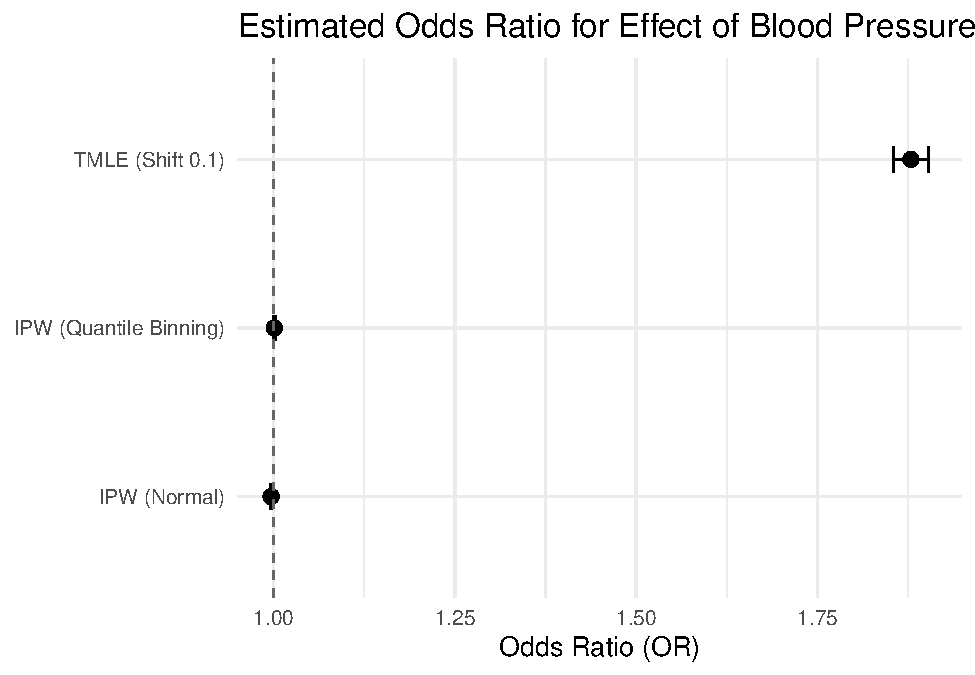
\includegraphics{rhc_analysis_files/figure-latex/forest-plot-or-1.pdf}

\begin{Shaded}
\begin{Highlighting}[]
\FunctionTok{library}\NormalTok{(knitr)}
\FunctionTok{library}\NormalTok{(kableExtra)}

\CommentTok{\# Prepare table of OR estimates}
\NormalTok{results\_table }\OtherTok{\textless{}{-}}\NormalTok{ estimates }\SpecialCharTok{\%\textgreater{}\%}
  \FunctionTok{transmute}\NormalTok{(}
\NormalTok{    Method,}
    \AttributeTok{OR =} \FunctionTok{sprintf}\NormalTok{(}\StringTok{"\%.3f"}\NormalTok{, OR),}
    \StringTok{\textasciigrave{}}\AttributeTok{95\% CI}\StringTok{\textasciigrave{}} \OtherTok{=} \FunctionTok{sprintf}\NormalTok{(}\StringTok{"\%.3f – \%.3f"}\NormalTok{, lower, upper),}
    \AttributeTok{SE =} \FunctionTok{sprintf}\NormalTok{(}\StringTok{"\%.3f"}\NormalTok{, SE)}
\NormalTok{  )}

\CommentTok{\# Show as styled table}
\FunctionTok{kable}\NormalTok{(results\_table, }\AttributeTok{format =} \StringTok{"latex"}\NormalTok{, }\AttributeTok{booktabs =} \ConstantTok{TRUE}\NormalTok{, }\AttributeTok{caption =} \StringTok{"Estimated Odds Ratios and 95\% Confidence Intervals"}\NormalTok{)}
\end{Highlighting}
\end{Shaded}

\textbackslash begin\{table\}

\textbackslash caption\{\label{tab:results-table}Estimated Odds Ratios
and 95\% Confidence Intervals\} \centering

\begin{tabular}[t]{llll}
\toprule
Method & OR & 95\% CI & SE\\
\midrule
IPW (Normal) & 0.997 & 0.996 – 0.997 & 0.000\\
IPW (Quantile Binning) & 1.001 & 0.999 – 1.002 & 0.001\\
TMLE (Shift 0.1) & 1.879 & 1.854 – 1.903 & 0.007\\
\bottomrule
\end{tabular}

\textbackslash end\{table\}

\subsection{Save plot}\label{save-plot}

\begin{Shaded}
\begin{Highlighting}[]
\CommentTok{\# Load required libraries}
\FunctionTok{library}\NormalTok{(ggplot2)}
\FunctionTok{library}\NormalTok{(patchwork)}

\CommentTok{\# Plot 1: Distribution of the exposure A (Blood Pressure)}
\NormalTok{p1 }\OtherTok{\textless{}{-}} \FunctionTok{ggplot}\NormalTok{(rhc, }\FunctionTok{aes}\NormalTok{(}\AttributeTok{x =}\NormalTok{ A)) }\SpecialCharTok{+}
  \FunctionTok{geom\_histogram}\NormalTok{(}\FunctionTok{aes}\NormalTok{(}\AttributeTok{y =}\NormalTok{ ..density..), }\AttributeTok{bins =} \DecValTok{40}\NormalTok{, }\AttributeTok{fill =} \StringTok{"grey70"}\NormalTok{, }\AttributeTok{color =} \StringTok{"black"}\NormalTok{) }\SpecialCharTok{+}
  \FunctionTok{geom\_density}\NormalTok{(}\AttributeTok{color =} \StringTok{"black"}\NormalTok{, }\AttributeTok{linewidth =} \DecValTok{1}\NormalTok{) }\SpecialCharTok{+}
  \FunctionTok{labs}\NormalTok{(}
    \AttributeTok{title =} \StringTok{"Distribution of Exposure: Blood Pressure"}\NormalTok{,}
    \AttributeTok{x =} \StringTok{"Mean Arterial Blood Pressure (mm Hg)"}\NormalTok{,}
    \AttributeTok{y =} \StringTok{"Density"}
\NormalTok{  ) }\SpecialCharTok{+}
  \FunctionTok{theme\_minimal}\NormalTok{(}\AttributeTok{base\_size =} \DecValTok{12}\NormalTok{)}

\CommentTok{\# Plot 2: Forest plot of estimated odds ratios for death}
\NormalTok{p2 }\OtherTok{\textless{}{-}} \FunctionTok{ggplot}\NormalTok{(estimates, }\FunctionTok{aes}\NormalTok{(}\AttributeTok{x =}\NormalTok{ Method, }\AttributeTok{y =}\NormalTok{ OR)) }\SpecialCharTok{+}
  \FunctionTok{geom\_point}\NormalTok{(}\AttributeTok{size =} \DecValTok{3}\NormalTok{, }\AttributeTok{color =} \StringTok{"black"}\NormalTok{) }\SpecialCharTok{+}
  \FunctionTok{geom\_errorbar}\NormalTok{(}\FunctionTok{aes}\NormalTok{(}\AttributeTok{ymin =}\NormalTok{ lower, }\AttributeTok{ymax =}\NormalTok{ upper), }\AttributeTok{width =} \FloatTok{0.15}\NormalTok{, }\AttributeTok{color =} \StringTok{"black"}\NormalTok{) }\SpecialCharTok{+}
  \FunctionTok{geom\_hline}\NormalTok{(}\AttributeTok{yintercept =} \DecValTok{1}\NormalTok{, }\AttributeTok{linetype =} \StringTok{"dashed"}\NormalTok{, }\AttributeTok{color =} \StringTok{"grey50"}\NormalTok{) }\SpecialCharTok{+}
  \FunctionTok{coord\_flip}\NormalTok{() }\SpecialCharTok{+}
  \FunctionTok{labs}\NormalTok{(}
    \AttributeTok{title =} \StringTok{"Estimated Association with In{-}Hospital Death"}\NormalTok{,}
    \AttributeTok{y =} \StringTok{"Odds Ratio (per 1 mm Hg increase in Blood Pressure)"}\NormalTok{,}
    \AttributeTok{x =} \ConstantTok{NULL}
\NormalTok{  ) }\SpecialCharTok{+}
  \FunctionTok{theme\_minimal}\NormalTok{(}\AttributeTok{base\_size =} \DecValTok{12}\NormalTok{)}

\CommentTok{\# Combine plots side by side}
\NormalTok{combined\_plot }\OtherTok{\textless{}{-}}\NormalTok{ p1 }\SpecialCharTok{+}\NormalTok{ p2 }\SpecialCharTok{+} \FunctionTok{plot\_layout}\NormalTok{(}\AttributeTok{ncol =} \DecValTok{2}\NormalTok{)}

\CommentTok{\# Display}
\FunctionTok{print}\NormalTok{(combined\_plot)}
\end{Highlighting}
\end{Shaded}

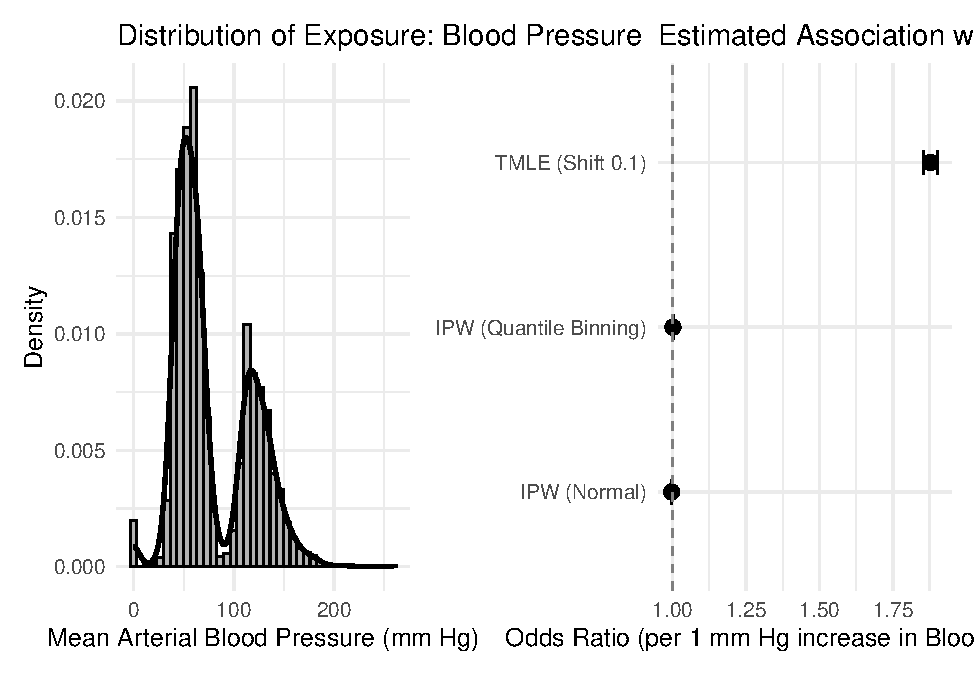
\includegraphics{rhc_analysis_files/figure-latex/save-plot-1.pdf}

\begin{Shaded}
\begin{Highlighting}[]
\CommentTok{\# Optional: Save the plot}
\FunctionTok{ggsave}\NormalTok{(}\StringTok{"rhc\_bw\_combined\_plot.png"}\NormalTok{, combined\_plot, }\AttributeTok{width =} \DecValTok{12}\NormalTok{, }\AttributeTok{height =} \DecValTok{5}\NormalTok{, }\AttributeTok{dpi =} \DecValTok{600}\NormalTok{)}
\end{Highlighting}
\end{Shaded}

\subsection{Diagnostic Checks}\label{diagnostic-checks}

To assess the reliability of causal estimates, we conduct several
diagnostic checks related to the validity of assumptions and model
performance. These include checking weight stability, covariate balance,
and the positivity assumption.

\subsubsection{Weight Diagnostics}\label{weight-diagnostics}

\begin{Shaded}
\begin{Highlighting}[]
\CommentTok{\# Histograms of weights}
\FunctionTok{summary}\NormalTok{(rhc}\SpecialCharTok{$}\NormalTok{sw\_normal)}
\end{Highlighting}
\end{Shaded}

\begin{verbatim}
##     Min.  1st Qu.   Median     Mean  3rd Qu.     Max. 
##   0.1041   0.7208   0.8650   1.0907   1.0737 243.6645
\end{verbatim}

\begin{Shaded}
\begin{Highlighting}[]
\FunctionTok{summary}\NormalTok{(rhc}\SpecialCharTok{$}\NormalTok{sw\_qbin)}
\end{Highlighting}
\end{Shaded}

\begin{verbatim}
##    Min. 1st Qu.  Median    Mean 3rd Qu.    Max. 
##  0.1136  0.5673  0.7700  1.0083  1.0925 22.7556
\end{verbatim}

\begin{Shaded}
\begin{Highlighting}[]
\FunctionTok{par}\NormalTok{(}\AttributeTok{mfrow =} \FunctionTok{c}\NormalTok{(}\DecValTok{1}\NormalTok{, }\DecValTok{2}\NormalTok{))}
\FunctionTok{hist}\NormalTok{(rhc}\SpecialCharTok{$}\NormalTok{sw\_normal, }\AttributeTok{main =} \StringTok{"IPW Normal Weights"}\NormalTok{, }\AttributeTok{xlab =} \StringTok{"Weight"}\NormalTok{, }\AttributeTok{col =} \StringTok{"grey80"}\NormalTok{, }\AttributeTok{border =} \StringTok{"white"}\NormalTok{)}
\FunctionTok{hist}\NormalTok{(rhc}\SpecialCharTok{$}\NormalTok{sw\_qbin, }\AttributeTok{main =} \StringTok{"IPW Quantile Binning Weights"}\NormalTok{, }\AttributeTok{xlab =} \StringTok{"Weight"}\NormalTok{, }\AttributeTok{col =} \StringTok{"grey80"}\NormalTok{, }\AttributeTok{border =} \StringTok{"white"}\NormalTok{)}
\end{Highlighting}
\end{Shaded}

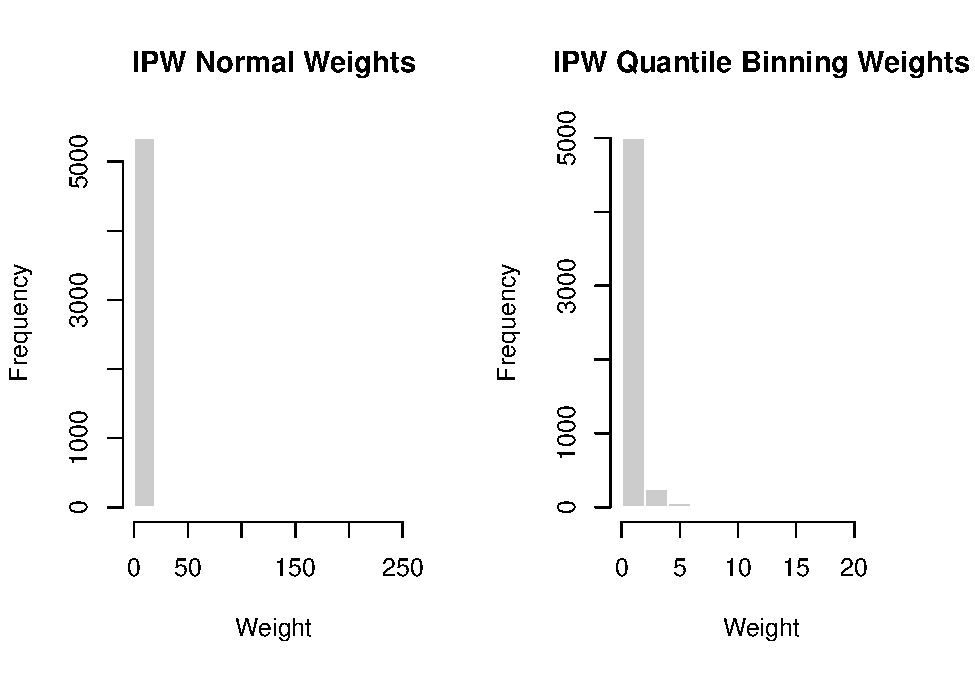
\includegraphics{rhc_analysis_files/figure-latex/weight-diagnostics-1.pdf}

Extreme or highly variable weights can indicate misspecification in the
exposure model or violations of the positivity assumption.

\subsubsection{Covariate Balance with
IPW}\label{covariate-balance-with-ipw}

\begin{Shaded}
\begin{Highlighting}[]
\CommentTok{\# Covariate balance before and after IPW using quantile binning}
\NormalTok{bal }\OtherTok{\textless{}{-}} \FunctionTok{bal.tab}\NormalTok{(}
  \FunctionTok{as.formula}\NormalTok{(}\FunctionTok{paste}\NormalTok{(}\StringTok{"A \textasciitilde{}"}\NormalTok{, }\FunctionTok{paste}\NormalTok{(covariates, }\AttributeTok{collapse =} \StringTok{" + "}\NormalTok{))),}
  \AttributeTok{data =}\NormalTok{ rhc,}
  \AttributeTok{weights =}\NormalTok{ rhc}\SpecialCharTok{$}\NormalTok{sw\_qbin,}
  \AttributeTok{method =} \StringTok{"weighting"}
\NormalTok{)}
\NormalTok{bal}
\end{Highlighting}
\end{Shaded}

\begin{verbatim}
## Balance Measures
##                      Type Corr.Adj
## age_[-Inf,50)      Binary  -0.0266
## age_[50,60)        Binary  -0.0026
## age_[60,70)        Binary   0.0167
## age_[70,80)        Binary   0.0173
## age_[80, Inf)      Binary  -0.0060
## sex_Female         Binary   0.0036
## Cardiovascular     Binary   0.0103
## Pulmonary          Binary   0.0020
## Renal              Binary   0.0079
## Congestive.HF      Binary  -0.0074
## Cancer_Metastatic  Binary   0.0068
## APACHE.score      Contin.  -0.0138
## DASIndex          Contin.   0.0013
## Albumin           Contin.   0.0116
## Creatinine        Contin.   0.0079
## Sodium            Contin.  -0.0454
## Heart.rate        Contin.  -0.0554
## WBC               Contin.   0.0001
## DNR.status_Yes     Binary   0.0149
## Transfer.hx        Binary  -0.0119
## 
## Effective sample sizes
##              Total
## Unadjusted 5351.  
## Adjusted   2382.93
\end{verbatim}

\begin{Shaded}
\begin{Highlighting}[]
\FunctionTok{love.plot}\NormalTok{(bal, }\AttributeTok{abs =} \ConstantTok{TRUE}\NormalTok{, }\AttributeTok{thresholds =} \FunctionTok{c}\NormalTok{(}\AttributeTok{m =} \FloatTok{0.1}\NormalTok{))}
\end{Highlighting}
\end{Shaded}

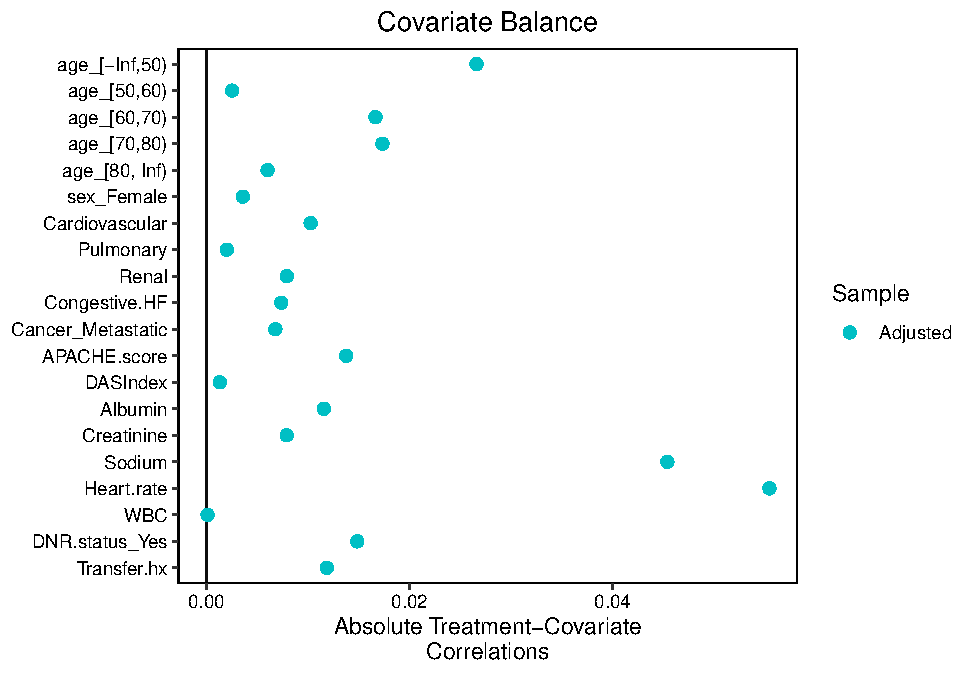
\includegraphics{rhc_analysis_files/figure-latex/covariate-balance-1.pdf}

The love plot shows performance before and after weighting. Good balance
is typically indicated by values below 0.1.

\subsubsection{Positivity Check}\label{positivity-check}

\begin{Shaded}
\begin{Highlighting}[]
\CommentTok{\# Exposure distribution by confounder category}
\FunctionTok{ggplot}\NormalTok{(rhc, }\FunctionTok{aes}\NormalTok{(}\AttributeTok{x =}\NormalTok{ A, }\AttributeTok{fill =}\NormalTok{ sex)) }\SpecialCharTok{+}
  \FunctionTok{geom\_density}\NormalTok{(}\AttributeTok{alpha =} \FloatTok{0.5}\NormalTok{) }\SpecialCharTok{+}
  \FunctionTok{labs}\NormalTok{(}\AttributeTok{title =} \StringTok{"Blood Pressure by Sex (as a Proxy for Positivity)"}\NormalTok{, }\AttributeTok{x =} \StringTok{"Blood Pressure"}\NormalTok{, }\AttributeTok{y =} \StringTok{"Density"}\NormalTok{) }\SpecialCharTok{+}
  \FunctionTok{theme\_minimal}\NormalTok{()}
\end{Highlighting}
\end{Shaded}

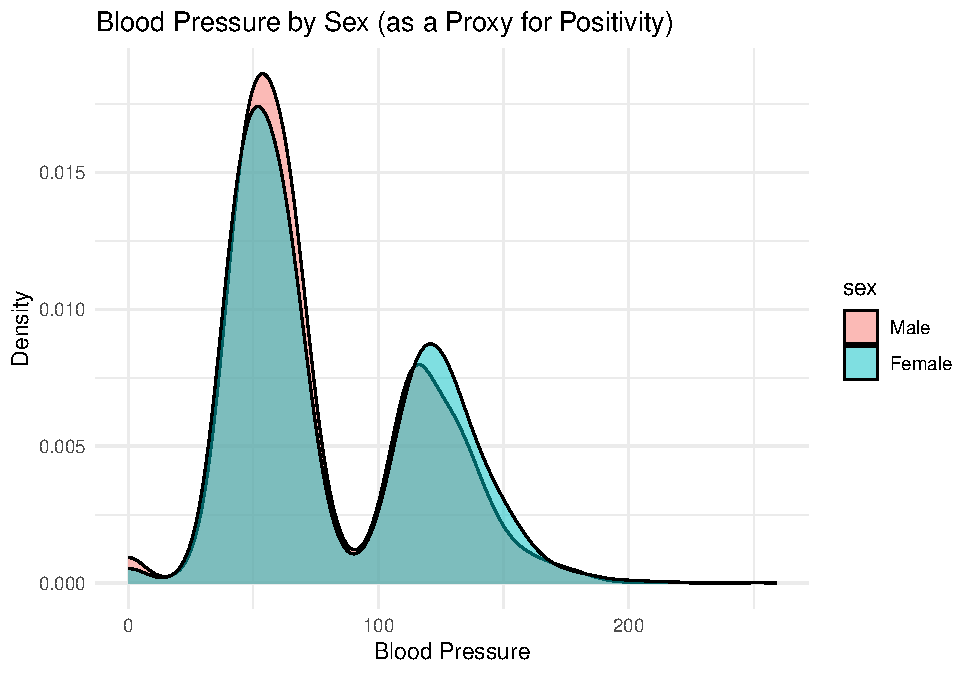
\includegraphics{rhc_analysis_files/figure-latex/positivity-check-1.pdf}

This density plot illustrates whether the exposure is sufficiently
variable across levels of key confounders. Lack of overlap may indicate
a positivity violation.

\end{document}
